\pagestyle{empty}
\frontmatter

%frontispiece
%\begin{figure*}[p]
%  	\centering
%  	\includegraphics[scale=0.2]{Durer/Albrecht_Dürer_The_Third_Knot.jpg}
%  	\caption{}
%  \end{figure*}
%\clearpage

\titleGM

\clearpage

%COPYRIGHT PAGE
\begin{vplace}[2]
\noindent
LA REVELACION DE JESUCRISTO: \\LEYENDO A LA LUZ DEL ANTIGUO TESTAMENTO\\
\newline
Copyright \copyright\ 2022 por Caleb George\\
Reservados todos los derechos.\\
\newline
Impreso en los Estados Unidos\\
\newline
Gracias por comprar una edición autorizada de este libro y por cumplir con las leyes de derechos de autor al no reproducir, escanear ni distribuir ninguna parte del mismo de ninguna forma sin permiso.
\newline
\newline
Primera Edición: Junio 2023
\newline
\newline
Las citas bíblicas identificadas (RVR 1960) han sido tomadas de la Reina-Valera 1960™ © Sociedades Bíblicas en América Latina, 1960. Derechos renovados 1988, Sociedades Bíblicas Unidas.
\newline
\newline
Kephali Press
\newline
Athens, AL 35613
\end{vplace}

\clearpage
\clearpage

\dedication
\clearpage

\ClearShipoutPicture
\AddToShipoutPicture{%
   \checkoddpage
   \transparent{0.1}
   \ifoddpage
     \put(0,0){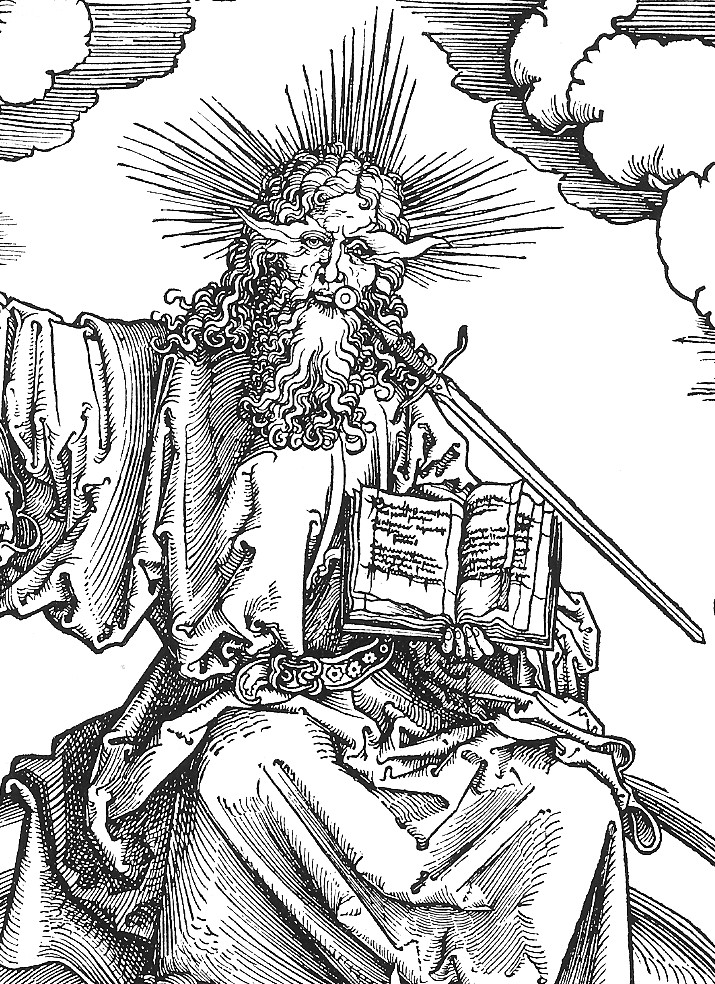
\includegraphics[width=\paperwidth,height=\paperheight]{Durer/Son_of_Man.jpg}}
   \else
     \put(0,0){\includegraphics[width=\paperwidth,height=\paperheight]{Durer/Dürer_Apocalypse_dragon.jpg}}
   \fi
}

\blankpage
\clearpage
\clearpage

\begin{KeepFromToc}
\tableofcontents
\end{KeepFromToc}
\clearpage
\listoffigures
\clearpage

%PREFACE
\chapter{Prefacio}
Hay dos cosas que yo y muchos otros hemos encontrado más útiles al estudiar el libro de Apocalipsis: (1) visualizar las cosas aterradoras y maravillosas que Jesús le mostró a Juan y (2) estudiar las conexiones entre el Apocalipsis y el Antiguo Testamento relevante. textos. Este libro está destinado a ayudar en ambos esfuerzos, pero especialmente en el último. \\

El Apocalipsis está repleto de citas y alusiones a la Biblia hebrea. La edición 28\textsuperscript{a} del Nuevo Testamento griego Nestlé-Aland incluye más de 700 referencias cruzadas del Antiguo Testamento en el libro de Apocalipsis. Recurrir físicamente a todas estas referencias en una copia impresa de la Biblia no es algo que el lector típico se incline a hacer. A los usuarios de teléfonos inteligentes o tabletas les puede resultar más fácil hacer clic en una referencia cruzada para ver un texto, pero incluso esto requiere un descanso en la concentración y puede implicar cambiar de ventana/página. El formato presentado en este libro le permite al lector echar un vistazo al final de una página e inmediatamente leer textos relevantes del AT, lo que le permite al usuario formar conexiones mentales rápidamente y profundizar su comprensión. Cada texto de referencia ha sido seleccionado cuidadosamente para brindar el mayor valor posible a los estudiantes de la Biblia y he tratado de brindar tanto contexto como lo permitan las limitaciones de espacio en la página. He evitado deliberadamente añadir comentarios e interpretaciones humanas; hay otros libros disponibles que lo hacen mejor que yo.\\

La literatura apocalíptica es muy visual. Los profetas Ezequiel, Daniel, Zacarías, etc. y el apóstol Juan usan repetidamente la frase “vi” (Ez. \ibiblechvs{Ezekiel}(1:1); Dan. \ibiblechvs{Daniel}(4:5 ); Zac. \ibiblechvs{Zechariah}(1:8); Rev. 1:12). Hacemos bien en tratar de ``ver'' las mismas cosas que vieron esos hombres; tenemos que ver la película antes de tratar de explicarlo. Fui bendecido en el grado 11\textsuperscript{th} de tener un maestro de Biblia, Steve Klein, quien realmente nos hizo dibujar las visiones en cada capítulo. Este ejercicio, independientemente de nuestra destreza artística, dio vida al texto. Por supuesto, el dibujo de una visión es una representación bidimensional de fotograma fijo de una experiencia dinámica tridimensional; e incluso para eso se requiere algo de imaginación y creatividad artística, ya que la visión nos fue transmitida en palabras que incluso los autores apocalípticos indican que eran inadecuadas para describir verdaderamente lo que vieron - nótese el uso frecuente de "me gusta" (Ap. 1 :13, 15; 2:18; 4:3, 6, 7, etc.). Pero tengo la esperanza de que los grabados en madera de Alberto Durero, que ahora tienen 524 años de antigüedad, en su gran \textit{Apocalipsis cum Figuris} estimulen su mente para mirar con Juan la gloria, la ira y la misericordia de Dios y del Cordero.\\

A Dios sea la gloria por brindar tan rica variedad de recursos destinados al estudio de su palabra. Es mi esperanza que este libro sea tan útil para usted como su preparación lo ha sido para mí. Quisiera agradecer a John Gibson por revisar un borrador inicial y proporcionar comentarios, a mis padres por su aliento y especialmente a mi querida esposa, Mabeliz, por su paciencia mientras pasaba muchas horas coloreando los grabados en madera píxel por píxel y escribiendo innumerables ajustes para el script \LaTeX{}. Este libro está amorosamente dedicado a ella.\\
\\
Caleb George\\
Managua, Nicaragua\\
Junio 2023
\clearpage

\cleartorecto
\begin{vplace}
\begin{center}
\textit{
¡Ay de mí! que soy muerto; \\
que siendo hombre inmundo de labios, \\
y habitando en medio de pueblo que tiene labios inmundos, \\
han visto mis ojos al Rey, \\
Jehová de los ejércitos.} \\
-ISAÍAS 6:5
\end{center}
\end{vplace}

\ClearShipoutPicture